

\documentclass[journal]{IEEEtran}
%\documentclass{article}
%\usepackage[]{natbib}
\usepackage{graphicx}
\usepackage{tikz}
\usepackage{mathtools}

% If IEEEtran.cls has not been installed into the LaTeX system files,
% manually specify the path to it like:
% \documentclass[journal]{../sty/IEEEtran}


\begin{document}
%
% paper title
% can use linebreaks \\ within to get better formatting as desired
\title{Experimental Evaluation of Control Policies for \\Segway Robot in Dynamic Environments }
\author{Ian~Buckley, Niharika~Arora, Varun~Murali}
\markboth{ECE6552, March 2016}%
{Shell \MakeLowercase{\textit{et al.}}: Project Proposal}
\maketitle
%%%%%%%%%%%%%%%%%%%%%%%%%%%%%%%%%%%%%%%%%%%%%%%%%%%%%%%%%%%%%%%%%%%%%%%%%%%%%%%%%%%%%%%%%%%%%%%

\begin{abstract}
\if0
Describe what the overall objectives are, the specific system being
considered.
\fi
With the growth of domestic robot industry, it is important to understand the navigation of mobile robots in dynamic environments. Use of mobile robots in the home can greatly improve the quality of life and is a growing field of research. An important aspect to be considered is the aspect of safety and guarantees that can be made about the safety of controllers on such robots. Given traditional digital control, mobile robot dynamics are often linearized to a setpoint and the controller is set to follow a point some distance \textbf{$d$} from the robot. The proposed study will attempt to characterize the stability of such a robotic system. We propose to study the applicability of barrier functions to prove the stability of the system given its set of constraints and the space it's allowed to operate in. The formulation of this problem in this form allows us to make claims about the stability of the control law, and study the conditions under which we can guarantee the success of the controller. The overall objective of the project is to apply barrier functions to generate a nonlinear control policy for a Segway RMP based robot.
\end{abstract}

\section{Introduction}
\if0
Motivate the problem being considered in a general way.  Use
this to setup the specific objectives of the project.  Give a high level overview
of the system that will be considered.  Finally, what are the concrete analy-
sis/control/safety objectives that will be met.
\fi

Navigation is a fundamental concern for mobile robots. The ability to successfully avoid obstacles, both static and dynamic, while moving towards a goal location largely determines the utility of a mobile robotic platform. It is important that robots avoid obstacles for their own safety as well as the safety of the people around them. Given the importance of navigation, it is not surprising that the problem has long been considered and explored; furthermore, it is reasonable to assert that approaches to the problem are as varied as the disciplines related to robotics themselves.  

In this paper, we propose to use nonlinear control techniques (barrier functions) for robot navigation and collision avoidance. We define constraints important for navigation like distance from obstacle, minimum and maximum velocity, minimum and maximum rotational velocity, and velocity as a function of distance from obstacle for safety to generate a navigation law for the robot.

Nonlinear control based navigation is also a studied problem such as by Ting et al. \cite{ting2014reactive}. Generating a policy in a reactive fashion reduces the complexity of the computation needed. Traditional path planners can be used to provide a high level trajectory by having some previous metric knowledge of the space. Lower level reactive controllers can be used for local refinement of the global path and can be used to control the robot. This reduces the complexity of re-planning every time a change in the environment is observed. Potential field based algorithms have been used to generate such reactive policies in the past with some success. There are some known pitfalls for this method with regards to local minima but several solutions for this have been proposed.

Given the possibility of having a global metric representation of a domestic environment, we could generate a global trajectory and local non-linear controller that obeys the bounds imposed on the robot.  If the barrier function comprises of the above information, we can make claims guarantees about the stability of the robot with respect to those objectives.

The navigation law will first be tested and verified in simulation. MATLAB will be used for this purpose. Once the simulations verify the algorithm, the controller will be implemented in the ROS framework and evaluated in a robot simulation environment (Gazebo). The final experiments will be performed on the mobile robot Jeeves, shown in Figure \ref{fig:jeeves}, which will be used as a test platform for the real world environment. We plan to study the law developed in both static and dynamic environments. 



\section{System Overview}
\if0
Discuss the system that will be considered. Indicate the
type of dynamics and phenomena it displays. Discuss how it will be analyzed
and how it will be used to set the stage for the overarching goals of the project.
Give a high level overview
of the system that will be considered. Finally, what are the concrete analysis/control/safety
objectives that will be met.
What are the specific objectives of the project, especially in the
context of the system of interest?
\fi
\begin{figure}
    \centering
    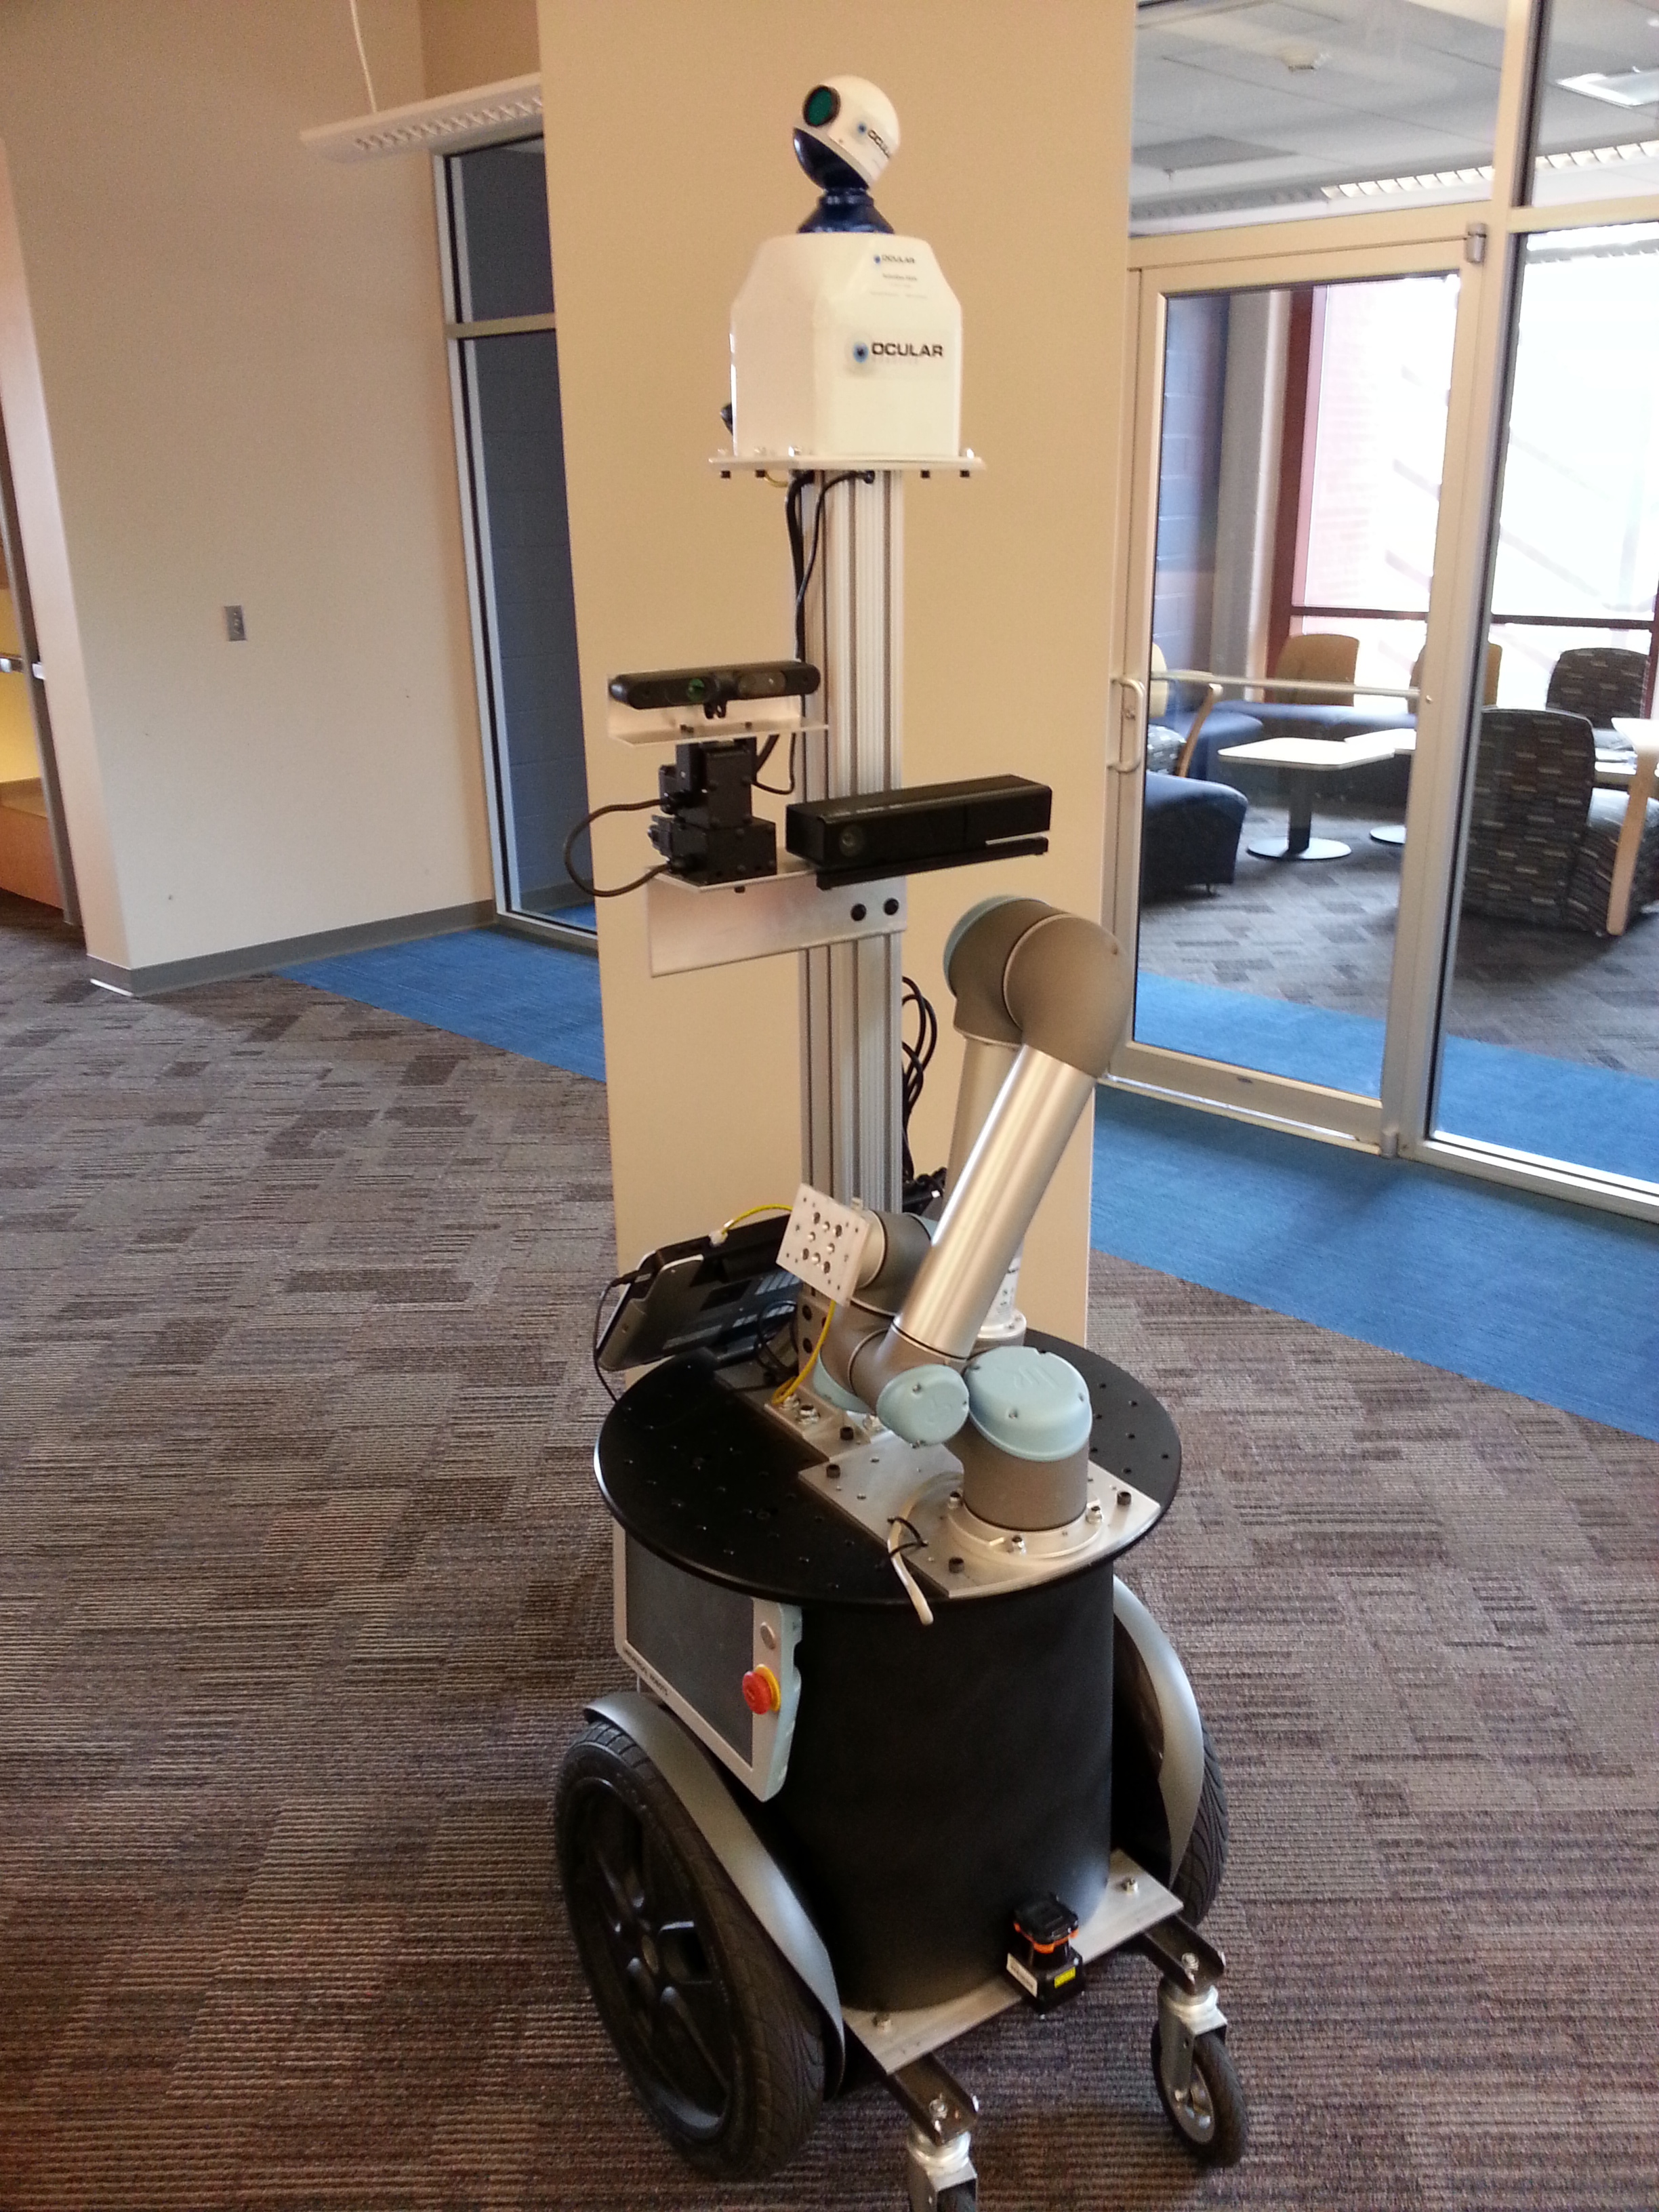
\includegraphics[width = 4cm, scale=0.2]{jeeves2_0.jpg}
    \caption{Jeeves - A modified Segway based robot mounted with a Primesense, Microsfot Kinect, Roboteye RE05, Hokuyo LTM-30x laser and the UR5. Currently modified to include the casters for static stability}
    \label{fig:jeeves}
\end{figure}

\begin{figure}
    \centering
    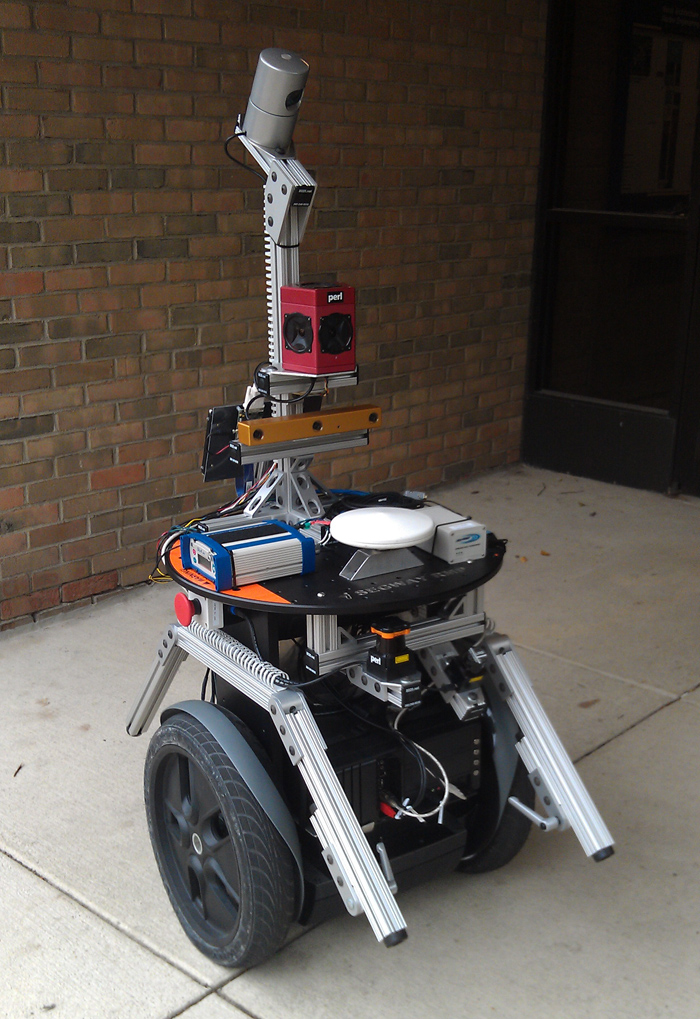
\includegraphics[width = 4cm, scale=0.2]{segway1.jpg}
    \caption{Proposed modification to the Segway base inspired by the Segway robot at the University of Michigan}
    \label{fig:mod_jeeves}
\end{figure}


The robot platform shown in Figure \ref{fig:jeeves} consists of a Segway RMP-200 mobile base, which has been
modified to hold various sensors. The Seqway RMP 200 has been modified to be statically stable but for the purposes of this project, the casters shall be removed and 8020 adjustments will be made on the side of the robot to prevent it from tipping (inspired by Figure \ref{fig:mod_jeeves}). The sensor suite on the robot consists of a Roboteye RE05 sensor capable of scanning in 3D, a primesense RGB-D camera and a Kinect RGB-D. The Hokuyo LTM-30x is mounted at the base and used for base obstacle avoidance. 

In the scope of this project, the Hokuyo LTM-30x is used to detect obstacles from a planar scan. The closest laser hit can be considered an obstacle and dynamic obstacles can be modelled in this way. A microstrain IMU is mounted on the robot to estimate the state of the robot.

The robot is controlled using a PS3 controller when in tele-operation mode, which has a manual override and a dead-man switch to kill the robot due to any type of failure. The robot is also permanently connected to a computer that is monitoring the robot and can be used to kill running programs on the robot.


The dynamics (discussed in \cite{castro2012modeling}) of the Segway RMP base can be modelled as a cart with an inverted pendulum which can be modelled as:

\begin{equation}
\centering
 mLsin(\theta)\dot{\theta}^2 + (M+m)\dot{v} - F - mLcos(\theta)\ddot{\theta} = 0 
\end{equation}

where $\theta$ is the angle of the pendulum with respect to its vertical position, $v$ is the speed of the base, $F$ is the force on the cart, $M$ is the mass of the cart and $m$ is the mass of the pendulum and $L$ is the length of the massless rod.

The control law will further be used to test how it affects the dynamics of the system. We will measure the translation and the rotational velocities and the tip angle to verify that the control policy doesn't force the robot to go beyond its boundary conditions and ensures its safety.


\section{Objective}
The objective of this project is to come up with a nonlinear control policy for navigation of mobile robots. To do this appropriate constraints have to be determined and specified. The initial constraints will be : 
\begin{itemize}
    \item The distance between the robotic platform and obstacles in the environment
    \item Minimum and maximum translational velocities of the robot
    \item Minimum and maximum angular velocities of the robot
\end{itemize}
These constraints will be used to generate a navigation controller for the Segway robot to ensure that the constraints are obeyed. Later, more constraints may be added to ensure safety of the robot and humans around the robot. The stability of the system with respect to the Lyapunov-like barrier functions will be analysed. This allows us to study theoretical guarantees of the controller for the Segway robot.

The experimental objective is to implement this controller on a real robot and study the gap between theory and practice in experimental scenarios. In the context of the system of interest, the nonlinear controller is used to study the robustness and stability of the generated control policy in the presence of obstacles in a real world scenario.

\section{Verification}
\if0
How will the objectives of the project be verified? Through
simulation, experimentally, formally, or through some combination of these?
Give specifics on how the individual objectives will be verified (in a concise
fashion).
\fi
\subsection{Simulation} 
The nonlinear control policy developed will be simulated in MATLAB to ensure expected behaviour of the algorithm and to evaluate it for different boundary conditions of the algorithm. The simulated environment will be shown as MATLAB GUI where the robot and obstacles are simulated and different randomized configurations of obstacles and several runs of the algorithm will be used to test the controller.
\subsection{Robot specific simulation}
The controller shall be implemented in the ROS framework and simulated using the Gazebo simulator for Jeeves. The simulation scenario would involve synthetic worlds and successful navigation in these worlds with the presence of introduced noise in the sensor reading and encoder measurement of the robot.

\subsection{Robot experiments}
Finally, the controller will be implemented on the Segway robot for experimental evaluation. The experimental evaluation will consist of five navigation test cases in which the robot will be instructed to navigate a static environment. Stability of the Segway will be examined for each test case and will be used to support the theoretical claims. The experiments will be performed in a motion capture room consisting of an 8 camera Optitrack system where the state of both obstacles and the robot can be measured. This will allow us to show the performance of the controller in the presence of both perfect and imperfect information. Further testing will include the addition of dynamic obstacles, such as people, to explore the capabilities of the proposed controller.

\bibliographystyle{IEEEtran}
\bibliography{IEEEabrv,bibi}

\end{document}